%%%%%%%%%%%%%%%%%%%%%%%%%%%%%%%%%%%%%%%%%%%%%%%%%%%%%%%%%%%%%%%%%%%%%%%%%%%%%%%%
% $Id: tg.tex 395 2015-10-02 14:22:13Z klugeflo $
%%%%%%%%%%%%%%%%%%%%%%%%%%%%%%%%%%%%%%%%%%%%%%%%%%%%%%%%%%%%%%%%%%%%%%%%%%%%%%%%
%%
%% Description of trace generation
%%
%%%%%%%%%%%%%%%%%%%%%%%%%%%%%%%%%%%%%%%%%%%%%%%%%%%%%%%%%%%%%%%%%%%%%%%%%%%%%%%%

\documentclass{article}

%%%%%%%%%%%%%%%%%%%%%%%%%%%%%%%%%%%%%%%%%%%%%%%%%%%%%%%%%%%%%%%%%%%%%%%%%%%%%%%%

\usepackage{algorithm}
%\usepackage{algorithmicx}
\usepackage{algpseudocode}
\usepackage{amsmath}
\usepackage{amssymb}
\usepackage[today]{svninfo}
\usepackage{tabularx}
\usepackage{textcomp}
\usepackage{todonotes}
\usepackage[normalem]{ulem}
\usepackage{xspace}

%%%%%%%%%%%%%%%%%%%%%%%%%%%%%%%%%%%%%%%%%%%%%%%%%%%%%%%%%%%%%%%%%%%%%%%%%%%%%%%%

\usepackage{tikz}
\usetikzlibrary{automata,calc,positioning}

%%%%%%%%%%%%%%%%%%%%%%%%%%%%%%%%%%%%%%%%%%%%%%%%%%%%%%%%%%%%%%%%%%%%%%%%%%%%%%%%
\makeatletter

\let\@textrightarrow=\textrightarrow
\def\textrightarrow{\@textrightarrow\xspace}

\def\eb{EMSBench\xspace}

\def\code#1{\texttt{#1}}

\makeatother
%%%%%%%%%%%%%%%%%%%%%%%%%%%%%%%%%%%%%%%%%%%%%%%%%%%%%%%%%%%%%%%%%%%%%%%%%%%%%%%%



%%%%%%%%%%%%%%%%%%%%%%%%%%%%%%%%%%%%%%%%%%%%%%%%%%%%%%%%%%%%%%%%%%%%%%%%%%%%%%%%



%%%%%%%%%%%%%%%%%%%%%%%%%%%%%%%%%%%%%%%%%%%%%%%%%%%%%%%%%%%%%%%%%%%%%%%%%%%%%%%%



%%%%%%%%%%%%%%%%%%%%%%%%%%%%%%%%%%%%%%%%%%%%%%%%%%%%%%%%%%%%%%%%%%%%%%%%%%%%%%%%
\begin{document}
%%%%%%%%%%%%%%%%%%%%%%%%%%%%%%%%%%%%%%%%%%%%%%%%%%%%%%%%%%%%%%%%%%%%%%%%%%%%%%%%

\svnInfo $Id: tg.tex 395 2015-10-02 14:22:13Z klugeflo $

\title{Trace Generation in \eb}
\author{Florian Kluge\\University of Augsburg}
\maketitle

%%%%%%%%%%%%%%%%%%%%%%%%%%%%%%%%%%%%%%%%%%%%%%%%%%%%%%%%%%%%%%%%%%%%%%%%%%%%%%%%

\begin{abstract}
  This document describes the model that underlies the trace generator
  of \eb.
\end{abstract}

%%%%%%%%%%%%%%%%%%%%%%%%%%%%%%%%%%%%%%%%%%%%%%%%%%%%%%%%%%%%%%%%%%%%%%%%%%%%%%%%

\tableofcontents

%%%%%%%%%%%%%%%%%%%%%%%%%%%%%%%%%%%%%%%%%%%%%%%%%%%%%%%%%%%%%%%%%%%%%%%%%%%%%%%%

%%%%%%%%%%%%%%%%%%%%%%%%%%%%%%%%%%%%%%%%%%%%%%%%%%%%%%%%%%%%%%%%%%%%%%%%%%%%%%%%
% $Id: parameters.tex 333 2015-06-30 13:00:39Z klugeflo $
%%%%%%%%%%%%%%%%%%%%%%%%%%%%%%%%%%%%%%%%%%%%%%%%%%%%%%%%%%%%%%%%%%%%%%%%%%%%%%%%

\section{Parameters}
\label{s:parameters}

%%%%%%%%%%%%%%%%%%%%%%%%%%%%%%%%%%%%%%%%%%%%%%%%%%%%%%%%%%%%%%%%%%%%%%%%%%%%%%%%

All parameters and associated units are depicted in
table~\ref{t:parameters}.
Please note that we use rounds (revolution of the crank shaft) as unit
for angular parameters to simplifie calculations.

%%%%%%%%%%%%%%%%%%%%%%%%%%%%%%%%%%%%%%%%%%%%%%%%%%%%%%%%%%%%%%%%%%%%%%%%%%%%%%%%

\subsection{Car Parameters}
\label{ss:parameters:car}

%%%%%%%%%%%%%%%%%%%%%%%%%%%%%%%%%%%%%%%%%%%%%%%%%%%%%%%%%%%%%%%%%%%%%%%%%%%%%%%%

%% # 195 / 70 R 14 86 H
%% #  a     b c d  e  f
%% a 175
%% b 65
%% d 15

%% # a = width
%% # b = aspect ratio
%% # d = diameter

\begin{table}
  \caption{Tyre labelling}
  \label{t:tyre}
  \centering
  \begin{tabular}{c@{/}ccccc}
    195 & 70 & R & 14 & 86 & H\\\hline
    $w$ & $r_t$ & - & $d_r$ & - & -
  \end{tabular}
\end{table}

\begin{itemize}
\item Tyres with (see also tab.~\ref{t:tyre}):
  \begin{itemize}
  \item Width $w$ [mm]
  \item Aspect ratio $r_t$ [\%]
  \item Rim diameter $d_r$ ["]
  \end{itemize}
\item Transmission ratio of cardan shaft and/or axle $r_a$
\item Transmission ratios of gears $\{G_1\ldots G_5\}$
\item idle speed of engine $U_I [\mbox{min}^{-1}]$
\item derived idle speed of engine:
  \begin{equation}
    \label{eq:omega:idle}
    \omega_I=\frac{U_I}{60}\frac{\mbox{min}}{\mbox{s}}
  \end{equation}

\end{itemize}

Calculation of tyre circumference:
\begin{itemize}
\item Flank height $h_f [\mbox{mm}]$ of tyre:
  \begin{equation}
    \label{eq:flank}
    h_f = w\frac{r}{100}
  \end{equation}
\item Wheel diameter $d_w [\mbox{mm}]$:
  \begin{equation}
    \label{eq:wdiam}
    d_w = 2.54\frac{\mbox{mm}}{\mbox{in}}d_r + 2h_f
  \end{equation}
\item Tyre circumference $C$:
  \begin{equation}
    \label{eq:tcirc}
    c_w = \pi d_w
  \end{equation}
\end{itemize}



%%%%%%%%%%%%%%%%%%%%%%%%%%%%%%%%%%%%%%%%%%%%%%%%%%%%%%%%%%%%%%%%%%%%%%%%%%%%%%%%

\subsection{Driving Cycle}
\label{ss:parameters:cycle}

%%%%%%%%%%%%%%%%%%%%%%%%%%%%%%%%%%%%%%%%%%%%%%%%%%%%%%%%%%%%%%%%%%%%%%%%%%%%%%%%

phase:
\begin{itemize}
\item acceleration $a [\frac{m}{s^2}]$
\item speed $v_s, v_e [\frac{km}{h}]$
\item duration $d [s]$
\item gear $g [0\ldots 5]$; gear $0$ stands for any time the engine is
  idle, i.e. when the clutch is pressed and thus disconnects the wheels from the engine.
\end{itemize}

Basic calculations:
\begin{itemize}
\item acceleration $\dot{\omega}_w$ of wheel (if $a\not=0$):
  \begin{equation}
    \dot{\omega}_w =
    \frac{a}{\frac{d_w}{1000}\frac{\mbox{m}}{\mbox{mm}}}
  \end{equation}
\item acceleration $\dot{\omega}_c$ of crank shaft (if $a\not=0$):
  \begin{equation}
    \dot{\omega}_c = \dot{\omega}_w G_g r_a
  \end{equation}
\end{itemize}

A simple example for a driving cycle is shown in table~\ref{t:cycle:example}.
Further examples can be found in appendix~\ref{s:dc}.

\begin{table}[htbp]
  \caption{Example for driving cycle (excerpt from urban cycle,
    operations 6-13)}
  \label{t:cycle:example}
  \begin{tabular}{c|l|c|c|c|c}
    Op. Nr. & Operation & Acc. & Speed & Dur. & Gear\\\hline
    1 & Idling & - & - & 21 & 16 s PM + 5 s K1\\
    2 & Acceleration & 0,83 & 0-15 & 5 & 1\\
    3 & Gear change & - & - & 2 & 1\textrightarrow2\\
    4 & Acceleration & 0,94 & 15-32 & 5 & 2\\
    5 & Steady speed & - & 32 & 24 & 2\\
    6 & Deceleration & -0,75 & 32-10 & 8 & 2\\
    7 & Dec., clutch diseng. & -0,92 & 10-0 & 3 & K2\\
    8 & Idling & - & - & 21 & 16 s PM + 5 s K1\\
  \end{tabular}
\end{table}

%%%%%%%%%%%%%%%%%%%%%%%%%%%%%%%%%%%%%%%%%%%%%%%%%%%%%%%%%%%%%%%%%%%%%%%%%%%%%%%%


%%%%%%%%%%%%%%%%%%%%%%%%%%%%%%%%%%%%%%%%%%%%%%%%%%%%%%%%%%%%%%%%%%%%%%%%%%%%%%%%

\begin{table}[htbp]
  \caption{Parameters used in trace generation}
  \label{t:parameters}
  \def\subt#1{\hline
    \multicolumn{4}{l}{\textbf{#1}}\\\hline
  }
  \begin{tabularx}{\textwidth}{l@{$\;:\ \;$}cc@{\quad}X}
    \multicolumn{1}{l}{\textbf{Symbol}} & \multicolumn{1}{l}{\textbf{Domain}} & \textbf{Unit} & \textbf{Description}\\
    \subt{Car}
    $w$ & $\mathbb{R}^+$ & mm & Tyre width\\\hline
    $r_t$ & $[1\ldots100]$ & \% & Aspect ratio flank/width\\\hline
    $d_r$ & $\mathbb{R}^+$ & in & Rim diameter\\\hline
    $r_a$ & $\mathbb{R}^+$ & - & Transmission ratio of cardan shaft
    and/or axle (input/output)\\\hline
    $g_{1\ldots5}$ & $\mathbb{R}^+$ & - & Transmission ratio of gears 1 to
    5 (input/output)\\\hline
    $U_I$ & $\mathbb{R}^+$ & $\mbox{min}^{-1}$ & Idle speed of
    engine\\\hline
    $\alpha_I$ & $\mathbb{R}^+$ & $\mbox{s}^{-2}$ & Absolute value of
    angular acceleration to reach idle speed when engine idle\\\hline
    \hline
    $\omega_I$ & $\mathbb{R}^+$ & $\mbox{s}^{-1}$ & Idle speed of
    engine (eq.~\eqref{eq:omega:idle})\\\hline
    $h_f$ & $\mathbb{R}^+$ & mm & Flank height of tyre (eq.~\eqref{eq:flank})\\\hline
    $d_w$ & $\mathbb{R}^+$ & mm & Wheel diameter (eq.~\eqref{eq:wdiam})\\\hline
    $c_w$ & $\mathbb{R}^+$ & mm & Tyre circumference (eq.~\eqref{eq:tcirc})\\\hline
    \subt{Rotary Sensor}
    $n_P$ & $\mathbb{N}$ & - & Number of primary teeth on rotary
    sensor\\\hline
    $n_S$ & $\mathbb{N}$ & - & Number of secondary teeth on rotary sensor\\\hline
    $O_P$ & $\{\mbox{abs},\mbox{pres}\}$ & - & Primary signal\\\hline
    $O_S$ & $\{\mbox{abs},\mbox{pres}\}$ & - & Secondary
    signal\\\hline
    $\Delta_P$ & $\mathbb{R}^+$ & (rounds) & Angular distance between
    two adjacent primary teeth\\\hline
    $\Delta_S$ & $\mathbb{R}^+$ & (rounds) & Angular distance between
    two adjacent secondary teeth\\\hline
    $\phi_S$ & $[3\Delta_P,4\Delta_P)$ & (rounds) & Angular distance
      between first primary and first secondary tooth; see \ref{p:trace:sectooth} for details\\\hline
    \subt{Driving Cycle}
    $a$ & $\mathbb{R}$ & $\mbox{m}\mbox{s}^{-2}$ &
    Acceleration\\\hline
    $v_s$ & $\mathbb{R}^+$ & $\mbox{km}\mbox{h}^{-1}$ & Car speed at
    start of operation\\\hline
    $v_e$ & $\mathbb{R}^+$ & $\mbox{km}\mbox{h}^{-1}$ & Car speed at
    end of operation\\\hline
    $d$ & $\mathbb{R}^+$ & s & Duration of operation\\\hline
    $g$ & $[0\ldots5]$ & - & Gear used in operation (0 = clutch disengaged)\\\hline
    \hline
    $\alpha_w$ & $\mathbb{R}$ & $\mbox{s}^{-2}$ & Angular acceleration
    of wheel\\\hline
    \subt{Crank Shaft Motion}
    $\varphi(t)$ & $\mathbb{R}^+_0$ & (rounds) & Angular position of crank
    shaft\\\hline
    $\omega(t)$ & $\mathbb{R}^+$ & $\mbox{s}^{-1}$ & Angular velocity
    of crank shaft\\\hline
    $\alpha$ & $\mathbb{R}$ & $\mbox{s}^{-2}$ & Angular acceleration
    of crank shaft\\\hline
  \end{tabularx}
\end{table}


%%%%%%%%%%%%%%%%%%%%%%%%%%%%%%%%%%%%%%%%%%%%%%%%%%%%%%%%%%%%%%%%%%%%%%%%%%%%%%%%


%%%%%%%%%%%%%%%%%%%%%%%%%%%%%%%%%%%%%%%%%%%%%%%%%%%%%%%%%%%%%%%%%%%%%%%%%%%%%%%%
%%% Local Variables: 
%%% mode: latex
%%% TeX-master: tg
%%% TeX-PDF-mode: t
%%% End: 
%%%%%%%%%%%%%%%%%%%%%%%%%%%%%%%%%%%%%%%%%%%%%%%%%%%%%%%%%%%%%%%%%%%%%%%%%%%%%%%%
%<!-- Local IspellDict: english -->

%%%%%%%%%%%%%%%%%%%%%%%%%%%%%%%%%%%%%%%%%%%%%%%%%%%%%%%%%%%%%%%%%%%%%%%%%%%%%%%%
% $Id: model.tex 333 2015-06-30 13:00:39Z klugeflo $
%%%%%%%%%%%%%%%%%%%%%%%%%%%%%%%%%%%%%%%%%%%%%%%%%%%%%%%%%%%%%%%%%%%%%%%%%%%%%%%%

\section{Model}
\label{s:model}

%%%%%%%%%%%%%%%%%%%%%%%%%%%%%%%%%%%%%%%%%%%%%%%%%%%%%%%%%%%%%%%%%%%%%%%%%%%%%%%%


%%%%%%%%%%%%%%%%%%%%%%%%%%%%%%%%%%%%%%%%%%%%%%%%%%%%%%%%%%%%%%%%%%%%%%%%%%%%%%%%

\subsection{Model Assumptions}

%%%%%%%%%%%%%%%%%%%%%%%%%%%%%%%%%%%%%%%%%%%%%%%%%%%%%%%%%%%%%%%%%%%%%%%%%%%%%%%%

\begin{itemize}
\item Ideal driver and engine: engine speed adapts exactly according
  to driving cycle
\item no car speed is lost while clutch is disengaged for gear change
\item FreeEMS NipponDenso uses 24/2 sensor at cam shaft which has half
  the speed of the crank shaft. Simplify model by assuming 12/1 sensor
  mounted to crank shaft, amounts to same behaviour
\item engine yields constant acceleration if accelerated/decelerated
\end{itemize}

%%%%%%%%%%%%%%%%%%%%%%%%%%%%%%%%%%%%%%%%%%%%%%%%%%%%%%%%%%%%%%%%%%%%%%%%%%%%%%%%

\subsection{Rotary Sensor}
\label{ss:model:rotary}

%%%%%%%%%%%%%%%%%%%%%%%%%%%%%%%%%%%%%%%%%%%%%%%%%%%%%%%%%%%%%%%%%%%%%%%%%%%%%%%%

Figure~\ref{f:rs} depicts the behaviour of the rotary sensor.
The automaton uses the current angular speed $\varphi(t)$ of the crank
shaft as input.
Any time a primary or secondary tooth passes a sensor, a
corresponding signal $O_p$ or $O_S$ is emitted.

\begin{figure}
  \centering
  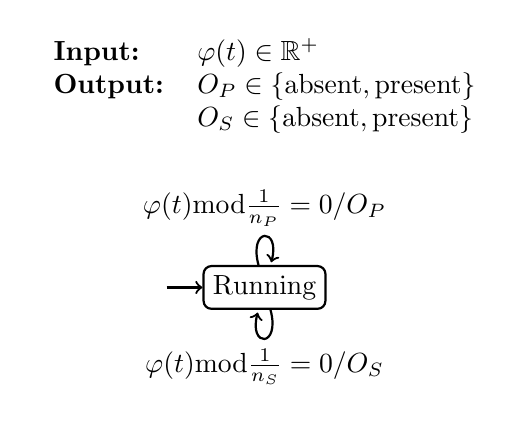
\begin{tikzpicture}[
      initial text={},%\begin{minipage}{1.5cm}$\omega_0:=\omega_L$\\$\varphi_0:=\alpha$\\$\alpha:=0$\end{minipage}},
      thick,node
      distance=1.5cm]
    \pgfsetcornersarced{\pgfpoint{1mm}{1mm}}
    \tikzstyle{state without output}=  [draw,every state,align=center]
    \node [state,initial] (running) {Running};

    \path %[transition]
    (running) edge [loop above] node [above] {$\varphi(t)\mbox{mod}\frac{1}{n_P}=0$/$O_P$} (running)
    (running) edge [loop below] node [below] {$\varphi(t)\mbox{mod}\frac{1}{n_S}=0$/$O_S$}(running)
    ;

    \node [above=of running] {
      \begin{tabular}{ll}
        \textbf{Input:} & $\varphi(t)\in\mathbb{R}^+$\\
        \textbf{Output:} & $O_P\in\{\mbox{absent},\mbox{present}\}$\\
        & $O_S\in \{\mbox{absent},\mbox{present}\}$
      \end{tabular}
    };
    
  \end{tikzpicture}
  \caption{Rotary Sensor}
  \label{f:rs}
\end{figure}


%%%%%%%%%%%%%%%%%%%%%%%%%%%%%%%%%%%%%%%%%%%%%%%%%%%%%%%%%%%%%%%%%%%%%%%%%%%%%%%%

\subsection{Crank Shaft}
\label{ss:model:crank}

%%%%%%%%%%%%%%%%%%%%%%%%%%%%%%%%%%%%%%%%%%%%%%%%%%%%%%%%%%%%%%%%%%%%%%%%%%%%%%%%

The behaviour of the crank shaft is depicted in figure~\ref{f:cs}.
The model develops the angular position $\varphi(t)$ and the angular
velocity $\omega(t)$.
Speed changes are managed through the angular acceleration
$\alpha$ which can be changed through the $\alpha_N$
input.
If a new $\alpha$ is set, the currently developed position and
speed are saved as new initial values, and the current time is stored
as new time offset.
Setting of $\alpha$ must ensure that the angular velocity
$\omega(t)$ never drops below $0$ (not contained in the model).

\begin{figure}
  \centering
  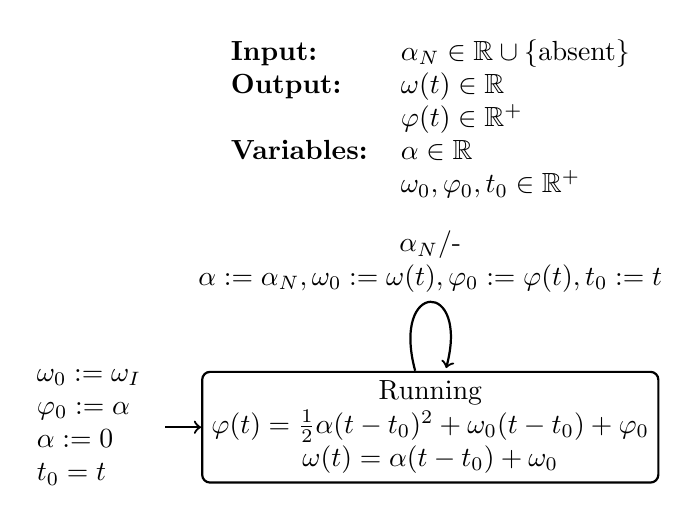
\begin{tikzpicture}[initial
      text={\begin{minipage}{1.5cm}$\omega_0:=\omega_I$\\$\varphi_0:=\alpha$\\$\alpha:=0$\\$t_0=t$\end{minipage}},thick,node
      distance=2.0cm]
    \pgfsetcornersarced{\pgfpoint{1mm}{1mm}}
    \tikzstyle{state without output}=  [draw,every state,align=center]
    \node [state,initial] (running) {Running\\
      $\varphi(t)=\frac{1}{2}\alpha(t-t_0)^2+\omega_0(t-t_0)+\varphi_0$\\
      $\omega(t)=\alpha(t-t_0)+\omega_0$
    };

    \path %[transition]
    (running) edge [loop above] node [above,align=center] {
      $\alpha_N$/-\\
      $\alpha:=\alpha_N, \omega_0:=\omega(t),
      \varphi_0:=\varphi(t),t_0:=t$
    } (running);

    \node [above=of running] {
      \begin{tabular}{ll}
        \textbf{Input:} & $\alpha_N\in\mathbb{R}\cup\{\mbox{absent}\}$\\
        \textbf{Output:} & $\omega(t)\in\mathbb{R}$\\
        & $\varphi(t)\in\mathbb{R}^+$\\
        \textbf{Variables:} & $\alpha\in\mathbb{R}$\\
        & $\omega_0,\varphi_0,t_0\in\mathbb{R}^+$\\
      \end{tabular}
    };
  \end{tikzpicture}
  \caption{Crank shaft behaviour}
  \label{f:cs}
\end{figure}

%%%%%%%%%%%%%%%%%%%%%%%%%%%%%%%%%%%%%%%%%%%%%%%%%%%%%%%%%%%%%%%%%%%%%%%%%%%%%%%%

\subsection{Determination of $\alpha$}
\label{ss:model:dotomega}

%%%%%%%%%%%%%%%%%%%%%%%%%%%%%%%%%%%%%%%%%%%%%%%%%%%%%%%%%%%%%%%%%%%%%%%%%%%%%%%%

Only under certain circumstances, accelerations $a$ of the car from a
driving cycle can be translated directly into angular accelerations of
the crank shaft.
There are a number of special situations, that also require some more
work.
Basically, we can describe the behaviour of the crank shaft as
consisting of phases with constant angular acceleration.
Each phase is a tuple $(\alpha,d)$ where $\alpha$ is the acceleration
of this phase, and $d$ is its duration.

%%%%%%%%%%%%%%%%%%%%%%%%%%%%%%%%%%%%%%%%%%%%%%%%%%%%%%%%%%%%%%%%%%%%%%%%%%%%%%%%

\subsubsection{Regular Operation}

A regular operation is on hand, if (1) the acceleration during an
operation is constant, and (2) there is no gear change during the
operation.
These condition is fulfilled by the following operations of a driving
cycle: \emph{idling}, \emph{steady speed}, \emph{deceleration}.
Additionally, if an \emph{acceleration} operation has a start speed
$\not=0$, it is also considered as a regular operation.

\paragraph{Idling}
\begin{equation}
  \label{eq:alpha:idling}
  \alpha = \alpha_I
\end{equation}


\paragraph{Steady Speed}
\begin{equation}
  \label{eq:alpha:steady}
  \alpha = 0
\end{equation}

\paragraph{Acceleration and Deceleration}
\begin{equation}
  \label{eq:alpha:ac-deceleration}
  \alpha = r_ag_i\frac{a}{c_w}\frac{1000\mbox{mm}}{\mbox{m}}
\end{equation}


%%%%%%%%%%%%%%%%%%%%%%%%%%%%%%%%%%%%%%%%%%%%%%%%%%%%%%%%%%%%%%%%%%%%%%%%%%%%%%%%

\subsubsection{Driveaway from Standstill}
\label{sss:model:driveaway}

Actual behaviour: Driver slowly releases clutch, may press
accelerator pedal.

Modeling: Simplify! Assume engine speed is constant (idle speed) until
clutch closed, then increases according to acceleration. Use
acceleration to calculate time until clutch closed (where engine idle speed
matches car speed).

relationship car speed $\leftrightarrow$ engine speed:
\begin{equation}
  \omega(t) = r_ag_i\frac{v(t)}{\frac{c_w}{1000}\frac{\mbox{m}}{\mbox{mm}}}
\end{equation}
with
\begin{equation}
  v(t) = at + v_0
\end{equation}

Now we need to find the time $t_I$ with $\omega(t_I) = \omega_I$.

Thus solve for $t$:
\begin{equation}
  r_ag_i\frac{at_I + v_0}{\frac{c_w}{1000}\frac{m}{mm}} = \omega_I
\end{equation}
with $v_0=0$ due to standstill, we get:
\begin{equation}
  \label{eq:driveaway:time}
  t_I = \frac{\omega_I}{r_ag_ia}\frac{c_w}{1000}\frac{m}{mm}
\end{equation}

Thus, we have a first phase of duration $t_I$ according to
eq.~\ref{eq:driveaway:time} where $\alpha=0$ and $\omega(t)=\omega_I$.
In in the second phase, $\alpha$ is calculated according to
eq.~\ref{eq:alpha:ac-deceleration}.

%%%%%%%%%%%%%%%%%%%%%%%%%%%%%%%%%%%%%%%%%%%%%%%%%%%%%%%%%%%%%%%%%%%%%%%%%%%%%%%%

\subsubsection{Gear Change}
\label{sss:model:gearchange}

Actual behaviour: driver presses clutch and releases accelarator pedal,
changes gear, releases clutch and presses accelerator.

Modeling: Split gear change operation in two phases with equal
duration.
Let $d_g$ be the total duration of the gear change operation.
Then each phase has a duration of $\frac{d_g}{2}$.
\begin{enumerate}
\item \textbf{Disengagement of clutch:}
  Assume that clutch and accelerator pedal are disengaged instantly at
  the beginning of this phase.
  Then, $\omega$ changes with $\alpha_I$ until $\omega_I$ reached or
  end of phase is reached.
  Depending on the initial angular velocity $\omega_0$, the angular acceleration
  must be chosen as:
  \begin{equation}
    \label{eq:alpha:gear:diseng}
    \alpha_g = \left\{
      \begin{array}{c@{\;:\;}l}
        -\alpha_I&\omega_0>\omega_I\\
        0 & \omega_0=\omega_I\\
        \alpha_I&\omega_0<\omega_I
      \end{array}
      \right.
  \end{equation}
  Angular velocity develops as:
  \begin{equation}
    \label{eq:omega}
    \omega(t) = \omega_0 + \alpha_g t
  \end{equation}
  Assume that phase starts at $t=0$. Distinguish \underline{two} cases:
  \begin{enumerate}
  \item If there exists a $t_I<\frac{d_g}{2}$ such that $\omega(t_I)=\omega_I$,
    introduce two phases $(\alpha_g,t_I)$, $(0,\frac{d_g}{2}-t_I)$.
  \item If no such $t_I$ exists, introduce \underline{one} phase $(\alpha,\frac{d_g}{2})$.
  \end{enumerate}
\item \textbf{Engagement of clutch with new gear:}
  Assume that the gear is changed at the beginning of this phase, and
  the clutch is finally closed exactly at the end of this phase.
  The aim is to develop $\omega(t)$ in such a manner that
  $\omega(d_g)$ matches the new rotation speed at the end of the
  phase.
  To simplify calculations, we renormalise the time base to $t=0$ at
  the beginning of the phase, and let $\omega_0$ be the angular
  velocity at the end of the previous phase.
  Let $v$ be the current speed of the car ($v_e$ of previous and $v_s$
  of next phase).
  Then, the target angular speed $\omega(\frac{d_g}{2})$ is
  \begin{equation}
    \omega(\frac{d_g}{2}) =
    r_ag_i\frac{v}{\frac{c_w}{1000}\frac{\mbox{m}}{\mbox{mm}}}
  \end{equation}
  Then, $\alpha_G$ is calculated as
  \begin{equation}
    \label{eq:omega:gear}
    \alpha_G = \frac{2}{d_g}\left(\omega(\frac{d_g}{2}) -
    \omega_0\right)
    =
    \frac{2}{d_g}\left(r_ag_i\frac{v}{\frac{c_w}{1000}\frac{\mbox{m}}{\mbox{mm}}}
    -\omega_0\right)
  \end{equation}

  %% gear change at beginning, $\omega$ must change such that it
  %% matches new (rotation) speed when clutch closed at end of phase.
  %% Need to find $\alpha_G$ such that
  %% \begin{equation}
  %%   \omega(t) = \omega_0 + \alpha_Gt
  %% \end{equation}
  %% with
  %% \begin{equation}
  %%   \omega(t) = \frac{v(t)}{\frac{d_w}{1000}\frac{m}{mm}}
  %% \end{equation}
  %% with $t$ end of phase. Solving for $\alpha_G$:
  %% \begin{equation}
  %%   \label{eq:omega:gear}
  %%   \alpha_G = \frac{1}{t}\left(\frac{v(t)}{\frac{d_w}{1000}\frac{m}{mm}} - \omega_0\right)
  %% \end{equation}
\end{enumerate}

Further assume that no speed is lost while clutch is disengaged.

%%%%%%%%%%%%%%%%%%%%%%%%%%%%%%%%%%%%%%%%%%%%%%%%%%%%%%%%%%%%%%%%%%%%%%%%%%%%%%%%

\subsubsection{Deceleration with Clutch Disengaged}
\label{sss:model:clutchdisen}

When the car is decelerated with the clutch being disengaged, the
engine speed should approximate $\omega_I$.
Let $d_d$ be the total duration of this operation.
We model this operation with two phases:
\begin{enumerate}
\item\textbf{Approximation:}
  If $\omega(t)=\omega_I$, this phase is skipped.
  Else, the engine speed has to drop or rise to $\omega_I$.
  Therefore, $\alpha_d$ is chosen according to
  eq.~\ref{eq:alpha:gear:diseng}.
  Again, assume that this phase starts at $t=0$.
  Then, the phase ends at $t_a$ with:
  \begin{equation}
    \omega(t_a) = \omega_I
  \end{equation}
  Combine with eq.~\ref{eq:omega} and solve for $t_a$ and add phase
  $(\alpha_d,\min(t_a,d_d))$.
  
\item\textbf{Idling:}
  If $t_a\geq d_d$, this phase is skipped.
  Else, the engine speed stays constant.
  We add a phase $(0, d_d-t_a)$.
\end{enumerate}

%%%%%%%%%%%%%%%%%%%%%%%%%%%%%%%%%%%%%%%%%%%%%%%%%%%%%%%%%%%%%%%%%%%%%%%%%%%%%%%%


%%%%%%%%%%%%%%%%%%%%%%%%%%%%%%%%%%%%%%%%%%%%%%%%%%%%%%%%%%%%%%%%%%%%%%%%%%%%%%%%


%%%%%%%%%%%%%%%%%%%%%%%%%%%%%%%%%%%%%%%%%%%%%%%%%%%%%%%%%%%%%%%%%%%%%%%%%%%%%%%%


%%%%%%%%%%%%%%%%%%%%%%%%%%%%%%%%%%%%%%%%%%%%%%%%%%%%%%%%%%%%%%%%%%%%%%%%%%%%%%%%


%%%%%%%%%%%%%%%%%%%%%%%%%%%%%%%%%%%%%%%%%%%%%%%%%%%%%%%%%%%%%%%%%%%%%%%%%%%%%%%%


%%%%%%%%%%%%%%%%%%%%%%%%%%%%%%%%%%%%%%%%%%%%%%%%%%%%%%%%%%%%%%%%%%%%%%%%%%%%%%%%


%%%%%%%%%%%%%%%%%%%%%%%%%%%%%%%%%%%%%%%%%%%%%%%%%%%%%%%%%%%%%%%%%%%%%%%%%%%%%%%%


%%%%%%%%%%%%%%%%%%%%%%%%%%%%%%%%%%%%%%%%%%%%%%%%%%%%%%%%%%%%%%%%%%%%%%%%%%%%%%%%


%%%%%%%%%%%%%%%%%%%%%%%%%%%%%%%%%%%%%%%%%%%%%%%%%%%%%%%%%%%%%%%%%%%%%%%%%%%%%%%%
%%% Local Variables: 
%%% mode: latex
%%% TeX-master: tg
%%% TeX-PDF-mode: t
%%% End: 
%%%%%%%%%%%%%%%%%%%%%%%%%%%%%%%%%%%%%%%%%%%%%%%%%%%%%%%%%%%%%%%%%%%%%%%%%%%%%%%%
%<!-- Local IspellDict: english -->

%%%%%%%%%%%%%%%%%%%%%%%%%%%%%%%%%%%%%%%%%%%%%%%%%%%%%%%%%%%%%%%%%%%%%%%%%%%%%%%%
% $Id: trace.tex 333 2015-06-30 13:00:39Z klugeflo $
%%%%%%%%%%%%%%%%%%%%%%%%%%%%%%%%%%%%%%%%%%%%%%%%%%%%%%%%%%%%%%%%%%%%%%%%%%%%%%%%

\section{Trace Generation}
\label{s:tracegen}

%%%%%%%%%%%%%%%%%%%%%%%%%%%%%%%%%%%%%%%%%%%%%%%%%%%%%%%%%%%%%%%%%%%%%%%%%%%%%%%%

%%%%%%%%%%%%%%%%%%%%%%%%%%%%%%%%%%%%%%%%%%%%%%%%%%%%%%%%%%%%%%%%%%%%%%%%%%%%%%%%

\subsection{Preliminary Considerations}
\label{ss:tracegen:prelim}

%%%%%%%%%%%%%%%%%%%%%%%%%%%%%%%%%%%%%%%%%%%%%%%%%%%%%%%%%%%%%%%%%%%%%%%%%%%%%%%%

Actual generation of traces on embedded platform should be as simple
as possible.
If enough memory is available, it would be possible to calculate all
signal times offline, such that the actual generator program simply runs
through a table.
Due to the vast memory requirements of such an approach, we utilise a
hybrid approach instead.
At least parts of the necessary calculations are performed offline.
Our aim is to implement trace generation through a composition of the
automatons described in sections~\ref{ss:model:rotary} and
\ref{ss:model:crank}.
Input data for these models is provided in pairs
$(t_N,\alpha_N)$, where $t_N$ is the time when the angular
acceleration changes to $\alpha_N$.

%%%%%%%%%%%%%%%%%%%%%%%%%%%%%%%%%%%%%%%%%%%%%%%%%%%%%%%%%%%%%%%%%%%%%%%%%%%%%%%%

\subsection{Preprocessor}
\label{ss:tracegen:preproc}

%%%%%%%%%%%%%%%%%%%%%%%%%%%%%%%%%%%%%%%%%%%%%%%%%%%%%%%%%%%%%%%%%%%%%%%%%%%%%%%%

The preprocessor transforms a driving cycle table (for examples, see
appendix~\ref{s:dc}) into an angular acceleration table for the actual
trace generator.
Thereby, the preprocessor proceeds as described in
section~\ref{ss:model:dotomega}.

%%%%%%%%%%%%%%%%%%%%%%%%%%%%%%%%%%%%%%%%%%%%%%%%%%%%%%%%%%%%%%%%%%%%%%%%%%%%%%%%

\subsection{Generator}
\label{ss:tracegen:generator}

%%%%%%%%%%%%%%%%%%%%%%%%%%%%%%%%%%%%%%%%%%%%%%%%%%%%%%%%%%%%%%%%%%%%%%%%%%%%%%%%

Tasks:
\begin{itemize}
\item set angular acceleration $\alpha$
\item develop $\varphi(t)$ and $\omega(t)$
\item generate signals $O_P, O_S$
\end{itemize}

Approach: Perform all relevant work in ISR for primary teeth.
Simplify implementation by setting a new $\alpha$ only when $O_P$
occurs.
$O_S$ timer is set in a corresponding (find an apt one) $O_P$
instance.
In the following, we use the expression \emph{phase} to denote the
time span between two changes of $\alpha$.
During a phase, $\alpha$ is constant.

%%%%%%%%%%%%%%%%%%%%%%%%%%%%%%%%%%%%%%%%%%%%%%%%%%%%%%%%%%%%%%%%%%%%%%%%%%%%%%%%

\subsubsection{Primary Teeth}

\begin{table}
  \caption{Parameters for primary teeth calculations}
  \label{t:parameters:primary}
  \vspace{1ex}
  \centering
  \begin{tabularx}{\textwidth}{c@{$\;:\ \;$}l@{\quad}X}
    \hline\hline
    $\Delta_P$ & $\mathbb{R}^+$ & Angular distance between two teeth\\
    $\varphi(t)$ & $\mathbb{R}^+_0$ & Angular position of crank shaft\\
    $\varphi^P_0$ & $\mathbb{R}^+_0$ & Initial position offset of
    crank shaft at beginning of current phase\\
    $\omega(t)$ & $\mathbb{R}^+_0$ & Angular velocity of crank shaft\\
    $\omega_0$ & $\mathbb{R}^+_0$ & Initial angular velocity of crank
    shaft at beginning of current phase\\
    $\alpha$ & $\mathbb{R} $ & Angular acceleration of crank
    shaft\\
    $t_0$ & $\mathbb{R}^+_0$ & Time offset of current phase\\
    \hline\hline
  \end{tabularx}
\end{table}

The parameters used in the following calculations are explained in
table~\ref{t:parameters:primary}.
The occurence of a primary tooth is characterised by the following
equation:
\begin{eqnarray}
  \varphi(t) - \varphi^P_0 \equiv 0 & (\mbox{mod } \Delta_P)
\end{eqnarray}
Through constraining a change of $\alpha$ to times where $O_P$
occurs, we can simplify this equation and search for the $k_P$-th
primary signal in a phase that is characterised by:
\begin{equation}
  \label{eq:trace:p:kth}
  \varphi(t) = \varphi^P_0 + k_P\Delta_P
\end{equation}

Solve equation~\eqref{eq:trace:p:kth}:
\begin{eqnarray}
  & \frac{1}{2}\alpha(t-t_0)^2+\omega_0(t-t_0)+\varphi^P_0 =
  \varphi^P_0 + k\Delta_P&\\
  \Leftrightarrow & \frac{1}{2}\alpha t^2 + \omega_0t -
  \frac{1}{2}\alpha t_0^2-\omega_0t_0 - k\Delta_P=0 &\\
  \Leftrightarrow & t_{1/2} = \frac{-\omega_0\pm\sqrt{\omega_0^2 +
      2\alpha\left(\frac{1}{2}\alpha t_0^2+\omega_0t_0 + k\Delta_P\right)}}{\alpha}&
\end{eqnarray}

We are only interested in the right-hand solution, as $t(k)$ must be a
monotonically increasing function:
\begin{equation}
  t(k) = \frac{-\omega_0 + \sqrt{\omega_0^2 +
      2\alpha\left(\frac{1}{2}\alpha t_0^2 +
      \omega_0t_0\right) + 2\alpha k\Delta_P}}{\alpha}
\end{equation}
Parts of the discriminant must only be calculated when a new
phase begins.
Defining two constants
\begin{eqnarray}
  D_1 & := & \omega_0^2 +
  2\alpha\left(\frac{1}{2}\alpha t_0^2 +
  \omega_0t_0\right)\\
  D_2 & := & 2\alpha\Delta_P
\end{eqnarray}
we can simplify $t(k)$:
\begin{equation}
  \label{eq:tk}
    t(k) = \frac{-\omega_0 + \sqrt{D_1 + D_2k}}{\alpha}
\end{equation}

The above calculations apply mainly to the primary signal $O_P$.
To generate $O_P$ concurrently, a closer look is necessary.
The basic approach is to perform all calculations only in the IRQ
handler of the $O_P$ routine.
Concerning $O_S$, a phase shift parameter
$\phi_S\in[0,\Delta_P)$ is introduced that describes the
angular distance betweeen the secondary tooth and the preceding
primary tooth.

%%%%%%%%%%%%%%%%%%%%%%%%%%%%%%%%%%%%%%%%%%%%%%%%%%%%%%%%%%%%%%%%%%%%%%%%%%%%%%%%

\subsubsection{Secondary Teeth}

\begin{table}
  \caption{Additional parameters for secondary teeth calculations}
  \label{t:parameters:secondary}
  \vspace{1ex}
  \centering
  \begin{tabularx}{\textwidth}{c@{$\;:\ \;$}l@{\quad}X}
    \hline\hline
    $\varphi^S_0$ & $\mathbb{R}^+_0$ & Initial position offset of next tooth\\
    $\Delta_S$ & $\mathbb{R}^+$ & Angular distance between two secondary teeth\\
    $\phi_S$ & $\mathbb{R}^+_0$ & Angular distance between next
    secondary tooth and primary tooth at which last phase change was triggered\\
    \hline\hline
  \end{tabularx}
\end{table}

Calculations of the secondary teeth times require additional
parameters that are summarised in table~\ref{t:parameters:secondary}.
Times for $O_S$ can be developed in a similar manner, but the
calculations will be a bit more complex, as a change of $\alpha$
will not necessarily overlap with an occurrence of $O_S$.
Thus, $O_S$ will occur any time when:
\begin{eqnarray}
  \varphi(t) - \varphi^S_0 \equiv 0 & (\mbox{mod } \Delta_S)
\end{eqnarray}
Ideally, the time of $O_S$ should just be calculated when the preceeding
primary tooth was triggered, to account for a possible change of
$\alpha$.

The $k$-th secondary signal in a single phase has the following
property:
\begin{equation}
  \label{eq:trace:s:kth}
  \varphi(t) = \varphi_0 + \phi_S + (k-1)\Delta_S
\end{equation}


%%%%%%%%%%%%%%%%%%%%%%%%%%%%%%%%%%%%%%%%%%%%%%%%%%%%%%%%%%%%%%%%%%%%%%%%%%%%%%%%

\subsubsection{Implementation Notes}

\paragraph{Time Units}
Use seconds.

\paragraph{Replace Multiplication by Addition}
Implementation should use equations~\eqref{eq:trace:p:kth} and
\eqref{eq:trace:s:kth}:
The $k$ parameter will only implicitly be kept, instead implementation
should simply advance the $k\Delta_P$ resp. $(k-1)\Delta_S$ products.

\paragraph{Keep Numbers small}
In the long rung, the angular position $\varphi(t)$ can grow to a very
large number.
Reset $\varphi(t)$ in regular intervals, e.g once per revolution, to
avoid loosing precision.

\paragraph{Irrelevance of Phase Shift}
For the use case, the initial phasing of the crank shaft is
irrelevant.
Therefore, set $\varphi_0:=0$.

\paragraph{Renormalisation}
Renormalisation is performed at $\varphi(t)=0\;(\mbox{mod }1)$.
\begin{eqnarray}
  \omega_0 & := & \omega(t)\\
  \varphi_0 & := & 0\\
  t_0 & := & t\\
  \leftrightarrow t & := & 0\\
\end{eqnarray}

\paragraph{Secondary Tooth}
\label{p:trace:sectooth}
Let the secondary tooth reside directly after the third primary tooth
at $\phi_S\in\left[3\Delta_P,4\Delta_P\right)$.

\paragraph{Phase Change}
May happen at any primary tooth.
Some phases are very short (1-2 teeth).
Restricting phase changes to only a single tooth would make the
discriminant in calculation of next $t$ (eq.~\eqref{eq:tk}) negative.
 Additional work:
\begin{equation}
  \alpha := \alpha_N
\end{equation}

\paragraph{Setting Secondary Tooth Timer}
Performed in ISR for second primary tooth.
Depending on the actual $\phi_S$, even the third ISR might suffice,
but we want to be on the safe side.

%%%%%%%%%%%%%%%%%%%%%%%%%%%%%%%%%%%%%%%%%%%%%%%%%%%%%%%%%%%%%%%%%%%%%%%%%%%%%%%%
%%% Local Variables: 
%%% mode: latex
%%% TeX-master: tg
%%% TeX-PDF-mode: t
%%% End: 
%%%%%%%%%%%%%%%%%%%%%%%%%%%%%%%%%%%%%%%%%%%%%%%%%%%%%%%%%%%%%%%%%%%%%%%%%%%%%%%%
%<!-- Local IspellDict: english -->

%%%%%%%%%%%%%%%%%%%%%%%%%%%%%%%%%%%%%%%%%%%%%%%%%%%%%%%%%%%%%%%%%%%%%%%%%%%%%%%%
% $Id: implementation.tex 395 2015-10-02 14:22:13Z klugeflo $
%%%%%%%%%%%%%%%%%%%%%%%%%%%%%%%%%%%%%%%%%%%%%%%%%%%%%%%%%%%%%%%%%%%%%%%%%%%%%%%%

\section{Implementation}
\label{s:implementation}

%%%%%%%%%%%%%%%%%%%%%%%%%%%%%%%%%%%%%%%%%%%%%%%%%%%%%%%%%%%%%%%%%%%%%%%%%%%%%%%%


%%%%%%%%%%%%%%%%%%%%%%%%%%%%%%%%%%%%%%%%%%%%%%%%%%%%%%%%%%%%%%%%%%%%%%%%%%%%%%%%

\subsection{Preprocessor}

%%%%%%%%%%%%%%%%%%%%%%%%%%%%%%%%%%%%%%%%%%%%%%%%%%%%%%%%%%%%%%%%%%%%%%%%%%%%%%%%


Algorithm~\ref{a:preprocessor} shows the basic structure/functionality
of the preprocessor tool.
The following special cases are handled:
\begin{description}
  \item[driveaway] is detected if the \emph{startspeed} of an
    operation is 0 and the \emph{endspeed} is $\not=0$.
  \item[standstill] \emph{start-} and \emph{endspeed} of the operation
    are 0
  \item[clutch disengaged] is found if the currend speed is $\not=0$
    and gear is 0.
  \item[gearchange] if the gear of the current phase is different from
    the one of the previous phase.
\end{description}



\begin{algorithm}
  \caption{Preprocessing of driving cycle}
  \label{a:preprocessor}
  \begin{algorithmic}
    \Require OperationList contains all operation of the driving
    cycle, each operation is a tuple (acceleration, startspeed,
    endspeed, duration, gear)
    \Ensure PhaseList contains the corresponding phases for the generator
    \Procedure{Preprocess}{OperationList}
    %\State \textbf{declare} PhaseList
    \ForAll{op in OperationList}
    \If{driveaway}
    \Comment{Phases according to sect.~\ref{sss:model:driveaway}}
    \State PhaseList.enqueue(0, $t$) \Comment{$t$ according to eq.~\eqref{eq:driveaway:time}}
    \State PhaseList.enqueue($\alpha_N$, op.duration$-t$)
    \ElsIf{standstill}
    \State PhaseList.enqueue($\pm\alpha_I$, $t$) \Comment{$t$
      until $\omega_I$ reached}
    \State PhaseList.enqueue(0, op.duration$-t$)
    \ElsIf{clutch disengaged}
    \Comment{Phases according to sect.~\ref{sss:model:clutchdisen}}
    \State PhaseList.enqueue($\pm\alpha_I$, $t$) \Comment{until
      $\omega_I$ reached}
    \State PhaseList.enqueue(0, op.duration$-t$)
    \ElsIf{gearchange}
    \Comment{Phases according to sect.~\ref{sss:model:gearchange}}
    \State PhaseList.enqueue($\pm\alpha_I$, $\frac{1}{2}$op.duration)
    \State PhaseList.enqueue($\alpha_G$,  $\frac{1}{2}$op.duration)
    \Comment{$\alpha_G$ from eq.~\eqref{eq:omega:gear}}
    \Else\Comment{regular driving/acceleration/deceleration}
    \State PhaseList.enqueue(angular acceleration, op.duration)
    \EndIf
    \EndFor
    \EndProcedure
  \end{algorithmic}
\end{algorithm}

%%%%%%%%%%%%%%%%%%%%%%%%%%%%%%%%%%%%%%%%%%%%%%%%%%%%%%%%%%%%%%%%%%%%%%%%%%%%%%%%

\subsection{Generator}

%%%%%%%%%%%%%%%%%%%%%%%%%%%%%%%%%%%%%%%%%%%%%%%%%%%%%%%%%%%%%%%%%%%%%%%%%%%%%%%%

The generator has to implement two interrupt service routines, one for
the primary tooth (alg.~\ref{a:isr:primary}) and one for the secondary
tooth (alg.~\ref{a:isr:secondary}).
Most of the work is performed in the primary ISR when the signal is
deactivated.

\begin{algorithm}
  \caption{ISR for primary tooth}
  \label{a:isr:primary}
  \begin{algorithmic}
    \Procedure{PrimaryISR}{}
    \If{pin activate}
    \State set deactivation time
    \State \Return
    \Else
    \If{$k==0$}\Comment{Renormalise}
    \State $\omega_0\gets\omega(t)$
    \State $\varphi_0\gets 0$
    \State $t\gets 0$
    \EndIf
    \If{phase change pending}\Comment{Change Phase}
    \State $\alpha\gets\alpha_N$
    \EndIf
    \State calculate next $t_P$
    \State set primary activation time
    \If{$k==1$}\Comment{set secondary timer}
    \State calculate next $t_S$
    \State set secondary activation time
    \EndIf
    \EndIf
    \EndProcedure
  \end{algorithmic}
\end{algorithm}

\begin{algorithm}
  \caption{ISR for secondary tooth}
  \label{a:isr:secondary}
  \begin{algorithmic}
    \Procedure{SecondaryISR}{}
    \If{pin activate}
    \State set deactivation time
    \State \Return
    \Else
    \Comment{do nothing}
    \EndIf
    \EndProcedure
  \end{algorithmic}
\end{algorithm}

The following constants are additionally necessary:
\begin{description}
\item[TimeToTicks] convert time values from solution of equations to
  timer ticks
\end{description}


Notes on implementation experience:
\begin{itemize}
\item Times for primary OC must be set relatively to previous primary
\item Times for secondary OC should be set absolutely.
  Using relative numbers would increase complexity.
  Absolute number should be derived from previous primary time
  (trigger of calculation).
\end{itemize}


%%%%%%%%%%%%%%%%%%%%%%%%%%%%%%%%%%%%%%%%%%%%%%%%%%%%%%%%%%%%%%%%%%%%%%%%%%%%%%%%


%%%%%%%%%%%%%%%%%%%%%%%%%%%%%%%%%%%%%%%%%%%%%%%%%%%%%%%%%%%%%%%%%%%%%%%%%%%%%%%%


%%%%%%%%%%%%%%%%%%%%%%%%%%%%%%%%%%%%%%%%%%%%%%%%%%%%%%%%%%%%%%%%%%%%%%%%%%%%%%%%


%%%%%%%%%%%%%%%%%%%%%%%%%%%%%%%%%%%%%%%%%%%%%%%%%%%%%%%%%%%%%%%%%%%%%%%%%%%%%%%%


%%%%%%%%%%%%%%%%%%%%%%%%%%%%%%%%%%%%%%%%%%%%%%%%%%%%%%%%%%%%%%%%%%%%%%%%%%%%%%%%
%%% Local Variables: 
%%% mode: latex
%%% TeX-master: tg
%%% TeX-PDF-mode: t
%%% End: 
%%%%%%%%%%%%%%%%%%%%%%%%%%%%%%%%%%%%%%%%%%%%%%%%%%%%%%%%%%%%%%%%%%%%%%%%%%%%%%%%
%<!-- Local IspellDict: english -->


%%%%%%%%%%%%%%%%%%%%%%%%%%%%%%%%%%%%%%%%%%%%%%%%%%%%%%%%%%%%%%%%%%%%%%%%%%%%%%%%

\clearpage
\begin{appendix}
  %%%%%%%%%%%%%%%%%%%%%%%%%%%%%%%%%%%%%%%%%%%%%%%%%%%%%%%%%%%%%%%%%%%%%%%%%%%%%%%%
% $Id: dc.tex 333 2015-06-30 13:00:39Z klugeflo $
%%%%%%%%%%%%%%%%%%%%%%%%%%%%%%%%%%%%%%%%%%%%%%%%%%%%%%%%%%%%%%%%%%%%%%%%%%%%%%%%

\section{Driving Cycle}
\label{s:dc}

%%%%%%%%%%%%%%%%%%%%%%%%%%%%%%%%%%%%%%%%%%%%%%%%%%%%%%%%%%%%%%%%%%%%%%%%%%%%%%%%

Tables~\ref{t:cycle:urban} and~\ref{t:cycle:extraurban} present
excerpts from "M6 COUNCIL DIRECTIVE
of 20 March 1970
on the approximation of the laws of the Member States on measures to be taken against air
pollution by emissions from motor vehicles" version from 01.01.2007.
These can be found in the files \verb+urban.ndc+
resp. \verb+extra-urban.ndc+ in the \verb+/data/+ directory.
The file \verb+nefz.ndc+ holds the whole driving cycle consisting of
four times the urban cycle and once the extra-urban cycle.


\begin{table}
  \caption{Urban cycle}
  \label{t:cycle:urban}
  \begin{tabular}{c|l|c|c|c|c}
    Op. Nr. & Operation & Acc. & Speed & Dur. & Gear\\\hline
    1 & Idling & - & - & 11 & 6 s PM + 5 s K1\\
    2 & Acceleration & 1,04 & 0-15 & 4 & 1\\
    3 & Steady speed & - & 15 & 9 & 1\\
    4 & Deceleration & -0,69 & 15-10 & 2 & 1\\
    5 & Dec., clutch diseng. & -0,92 & 10-0 & 3 & K1\\
    6 & Idling & - & - & 21 & 16 s PM + 5 s K1\\
    7 & Acceleration & 0,83 & 0-15 & 5 & 1\\
    8 & Gear change & - & - & 2 & 1\textrightarrow2\\
    9 & Acceleration & 0,94 & 15-32 & 5 & 2\\
    10 & Steady speed & - & 32 & 24 & 2\\
    11 & Deceleration & -0,75 & 32-10 & 8 & 2\\
    12 & Dec., clutch diseng. & -0,92 & 10-0 & 3 & K2\\
    13 & Idling & - & - & 21 & 16 s PM + 5 s K1\\
    14 & Acceleration & 0,83 & 0-15 & 5 & 1\\
    15 & Gear change & - & - & 2 & 1\textrightarrow2\\
    16 & Acceleration & 0,62 & 15-35 & 9 & 2\\
    17 & Gear change & - & - & 2 & 2\textrightarrow3\\
    18 & Acceleration & 0,52 & 35-50 & 8 & 3\\
    19 & Steady speed & - & 50 & 12 & 3\\
    20 & Deceleration & -0,52 & 50-35 & 8 & 3\\
    21 & Steady speed & - & 35 & 13 & 3\\
    22 & Gear change & - & - & 2 & 3\textrightarrow2\\
    23 & Deceleration & -0,86 & 35-10 & 7 & 2\\
    24 & Dec., clutch diseng. & -0,92 & 10-0 & 3 & K2\\
    25 & Idling & - & - & 7 & 7 s PM\\
  \end{tabular}
\end{table}


\begin{table}
  \caption{Extra-urban cycle}
  \label{t:cycle:extraurban}
  \begin{tabular}{c|l|c|c|c|c}
    Op. Nr. & Operation & Acc. & Speed & Dur. & Gear\\\hline
    1 & Idling & - & - & 20 & K1\\
    2 & Acceleration & 0,83 & 0-15 & 5 & 1\\
    3 & Gear change & - & - & 2 & 1\textrightarrow2\\
    4 & Acceleration & 0,62 & 15-35 & 9 & 2\\
    5 & Gear change & - & - & 2 & 2\textrightarrow3\\
    6 & Acceleration & 0,52 & 35-50 & 8 & 3\\
    7 & Gear change & - & - & 2 & 3\textrightarrow4\\
    8 & Acceleration & 0,43 & 50-70 & 13 & 4\\
    9 & Steady speed & - & 70 & 50 & 5\\
    10 & Deceleration & -0,69 & 70-50 & 8 & 4 s.5 + 4 s.4\\
    11 & Steady speed & - & 50 & 69 & 4\\
    12 & Acceleration & 0,43 & 50-70 & 13 & 4\\
    13 & Steady speed & - & 70 & 50 & 5\\
    14 & Acceleration & 0,24 & 70-100 & 35 & 5\\
    15 & Steady speed & - & 100 & 30 & 5*\\
    16 & Acceleration & 0,28 & 100-120 & 20 & 5*\\
    17 & Steady speed & - & 120 & 10 & 5*\\
    18 & Deceleration & -0,69 & 120-80 & 16 & 5*\\
    19 & Deceleration & -1,04 & 80-50 & 8 & 5*\\
    20 & Dec., clutch diseng. & -1,39 & 50-0 & 10 & K5\\
    21 & Idle & - & - & 20 & PM\\
  \end{tabular}
\end{table}


%%%%%%%%%%%%%%%%%%%%%%%%%%%%%%%%%%%%%%%%%%%%%%%%%%%%%%%%%%%%%%%%%%%%%%%%%%%%%%%%

%%% Local Variables: 
%%% mode: latex
%%% TeX-master: tg
%%% TeX-PDF-mode: t
%%% End: 

%%%%%%%%%%%%%%%%%%%%%%%%%%%%%%%%%%%%%%%%%%%%%%%%%%%%%%%%%%%%%%%%%%%%%%%%%%%%%%%%
%<!-- Local IspellDict: english -->

\end{appendix}

%%%%%%%%%%%%%%%%%%%%%%%%%%%%%%%%%%%%%%%%%%%%%%%%%%%%%%%%%%%%%%%%%%%%%%%%%%%%%%%%

%%%%%%%%%%%%%%%%%%%%%%%%%%%%%%%%%%%%%%%%%%%%%%%%%%%%%%%%%%%%%%%%%%%%%%%%%%%%%%%%
\end{document}
%%%%%%%%%%%%%%%%%%%%%%%%%%%%%%%%%%%%%%%%%%%%%%%%%%%%%%%%%%%%%%%%%%%%%%%%%%%%%%%%

%%% Local Variables: 
%%% mode: latex
%%% TeX-master: t
%%% TeX-PDF-mode: t
%%% End: 

%%%%%%%%%%%%%%%%%%%%%%%%%%%%%%%%%%%%%%%%%%%%%%%%%%%%%%%%%%%%%%%%%%%%%%%%%%%%%%%%
%<!-- Local IspellDict: english -->
